%\documentclass[mathserif]{beamer}
\documentclass[handout]{beamer}
%\usetheme{Goettingen}
\usetheme{Warsaw}
%\usetheme{Singapore}
%\usetheme{Frankfurt}
%\usetheme{Copenhagen}
%\usetheme{Szeged}
%\usetheme{Montpellier}
%\usetheme{CambridgeUS}
%\usecolortheme{}
%\setbeamercovered{transparent}
\usepackage[english, activeacute]{babel}
\usepackage[utf8]{inputenc}
\usepackage{amsmath, amssymb}
\usepackage{dsfont}
\usepackage{graphics}
\usepackage{cases}
\usepackage{graphicx}
\usepackage{pgf}
\usepackage{epsfig}
\usepackage{amssymb}
\usepackage{multirow}	
\usepackage{amstext}
\usepackage[ruled,vlined,lined]{algorithm2e}
\usepackage{amsmath}
\usepackage{epic}
\usepackage{epsfig}
\usepackage{fontenc}
\usepackage{framed,color}
\usepackage{palatino, url, multicol}
\usepackage{listings}
%\algsetup{indent=2em}


\vspace{-0.5cm}
\title{Markov Chain Monte Carlo}
\vspace{-0.5cm}
\author[Felipe Bravo Márquez]{\footnotesize
%\author{\footnotesize  
 \textcolor[rgb]{0.00,0.00,1.00}{Felipe José Bravo Márquez}} 
\date{ \today }




\begin{document}
\begin{frame}
\titlepage


\end{frame}


%%%%%%%%%%%%%%%%%%%%%%%%%%%


\begin{frame}{Markov Chain Monte Carlo}
\scriptsize{
\begin{itemize}
\item This class  introduces estimation of posterior probability distributions using a stochastic process known
as \textbf{Markov chain Monte Carlo} (MCMC). 

\item Here we'll produce samples from the joint posterior without maximizing anything. 

\item We will be able to sample directly from the posterior without assuming a Gaussian, or any other, shape. 

\item The cost of this power is that it may take much longer for our estimation to complete.

\item But the benefit is escaping multivariate normality assumption of the Laplace approximation.

\item More advanced models such as the generalized linear and multilevel models tend to produce non-Gaussian posterior distributions.

\item In most cases  they cannot
be estimated at all with the techniques of earlier classes. 


\item This class is based on Chapter 9 of \cite{mcelreath2020statistical} and Chapter 7 of \cite{kruschke2014doing}.
 
\end{itemize}



} 

\end{frame}




\begin{frame}{Markov Chain Monte Carlo}
\scriptsize{
\begin{itemize}
\item The essence of MCMC is to produce samples from the posterior $f(\theta|d)$ by only accessing a function that is proportial to it.
\item This proportial function is the product of the likelihood and the prior $f(d|\theta)*f(\theta)$, which is always available in a Bayesian model.
\item So, merely by evaluating $f(d|\theta)*f(\theta)$, without normalizing it by $f(d)$, MCMC allows us to generate random representative values from the posterior distribution.

\item This property is wonderful because the method obviates direct computation of the evidence $f(d)$, which, as you'll recall, is one of the most difficult aspects of Bayesian
inference. 

\item It has only been with the development of MCMC algorithms an software that Bayesian inference is applicable to complex data analysis.
\item And it has only been with the production of fast and cheap computer hardware that Bayesian inference is accessible to a wide audience.

\item The question then becomes this: How does MCMC work? For an answer, let's ask a politician. 
 
\end{itemize}



} 

\end{frame}




\begin{frame}{A politician stumbles upon the Metropolis algorithm}
\scriptsize{

\begin{itemize}
\item Suppose an elected politician lives on a long chain of islands.
\item He is constantly traveling from island to island, wanting to stay in the public eye. 
\item At the end of a day he has to decide whether to:

\begin{enumerate}
\scriptsize{
 \item stay on the current island
 \item move to the adjacent island to the left
 \item move to the adjacent island to right }
\end{enumerate}

\item His goal is to visit all the islands \textbf{proportionally} to their \textbf{relative population}.

\item But, he doesn't know the total population of all the islands.
\item He only knows the population of the current island where he is located.
\item He can also ask about the population of an adjacent island to which he plans to move.

\end{itemize}


} 
\end{frame}


\begin{frame}{The Metropolis algorithm}
\scriptsize{

\begin{itemize}
\item The politician has a simple heuristic for travelling accross the islands called the \textbf{Metropolis} algorithm \cite{metropolis1953equation}.

\item First, he flips a (fair) coin to decide whether to propose the adjacent island to the left or the adjacent island to the right.

\item If the proposed island has a larger population than
the current island ($P_{proposed}>P_{current}$), then he  goes to the proposed island.

\item If the proposed island has a smaller population than the current island ($P_{proposed}<P_{current}$), then he goes to the proposed island with probability $p_{move}=P_{proposed}/P_{current}$.


\item In the long run, the probability that the politician is on any one of the islands exactly matches the relative population of the island!

\end{itemize}


} 
\end{frame}


\begin{frame}{The Metropolis algorithm}
\scriptsize{

\begin{itemize}
\item Let's analyze the Metropolis algorithm in more detail.
\item Suppose there are 10 islands in total.
\item Each island is neighbored by two others, and the
entire archipelago forms a ring.
\item The islands are of different sizes, and so had different sized populations living on them.
\item The second island is twice as populous as the first,
the third three times as populous as the first.
\item And so on, up to the largest island, which is 10 times as populous as the smallest.

\end{itemize}


} 
\end{frame}


\begin{frame}{The Metropolis algorithm}

   \begin{figure}[h!]
	\centering
	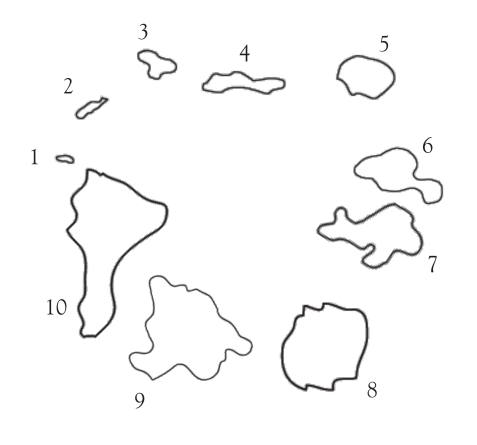
\includegraphics[scale=0.5]{pics/islands.png}
	\end{figure} 

\end{frame}




\begin{frame}{The Metropolis algorithm}
\scriptsize{

\begin{itemize}
\item We are going to show an implementation of this algorithm in R.

\item But before that, we will combine combine the two possibilities for the probability of moving into a single expression: the proposed island having a 1) higher or 2) lower population than the current island.

\begin{equation}
p_{move}=\min(1,P_{proposed}/P_{current}). 
\end{equation}

\item So, if $P_{proposed}>P_{current}$, $P_{proposed}/P_{current}>1$ and $p_{move}=1$.

\item For example, $current=4$ and $proposed=5$, $5/4>1$ so we move to the proposed island (with probability 1). 

\item On the other hand, if $P_{proposed}<P_{current}$, $P_{proposed}/P_{current}<1$, and $p_{move}=P_{proposed}/P_{current}$.

\item For example, $current=4$ and $proposed=3$, $3/4<1$ so we move to the proposed island with probability $3/4$.

\end{itemize}


} 
\end{frame}



\begin{frame}[fragile]{The Metropolis algorithm}
\scriptsize{


\begin{verbatim}
num_days <- 1e5
positions <- rep(0,num_days)
current <- 10
for ( i in 1:num_days ) {
  # record current position
  positions[i] <- current
  # flip coin to generate proposal
  proposal <- current + sample( c(-1,1) , size=1 )
  # now make sure he loops around the archipelago
  if ( proposal < 1 ) proposal <- 10
  if ( proposal > 10 ) proposal <- 1
  # move?
  prob_move <- min(proposal/current,1)
  decision <- rbinom(1,1,prob_move)
  current <- ifelse( decision == 1 , proposal , current )
}

library(rethinking)
simplehist(positions,xlab="island",ylab="number of days")
\end{verbatim}



} 
\end{frame}


\begin{frame}{The Metropolis algorithm}

   \begin{figure}[h!]
	\centering
	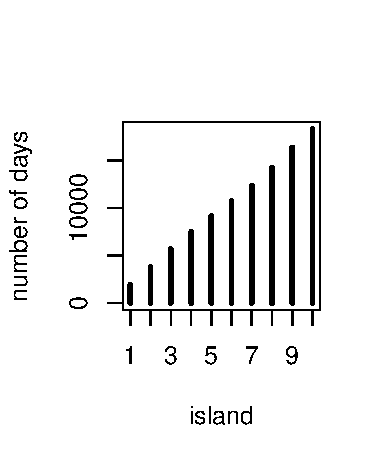
\includegraphics[scale=0.92]{pics/mcmc_islands.pdf}
	\end{figure} 

\scriptsize{
	The time spent on each island is proportional to its population size.}
	
\end{frame}



\begin{frame}{The Metropolis algorithm}
\scriptsize{

\begin{itemize}
\item The first three lines of the method just define
the number of days to simulate, an empty history vector, and a starting island position (the biggest island, number 10).
\item Then the for loop steps through the days. 
\item Each day, it records the politician's current position.
\item Then it simulates a coin flip to nominate a proposal island. 
\item The only trick here lies in making sure that a proposal of ``11'' loops around to island 1 and a proposal of “0” loops around to island 10.
\item Finally, a random binary number is generated with a Bernoulli distribution (Binomial with 1 trial) with probability of success (or moving)$=\min(1,P_{proposed}/P_{current})$.
\item If this random number is 1 we move, otherwise we stay.

\end{itemize}


} 
\end{frame}




\begin{frame}{The Metropolis algorithm}
\scriptsize{

\begin{itemize}
\item In real applications, the goal is not to help a politician, but instead to draw samples from an unknown and usually complex posterior probability distribution.
\item The ``islands'' in our objective are parameter values $\theta$, and they need not be discrete, but can instead take on a continuous range of values as usual.
\item The ``population sizes'' in our objective are the posterior probabilities (or densities) at each parameter value: $f(\theta|d)$
\item The ``days'' in our objective are samples taken from the posterior distribution.

\item The Metropolis algorithm will eventually give us a collection of samples from the posterior. 

\item We can then use these samples just like all the samples we have already used in this course.

\end{itemize}


} 
\end{frame}



\begin{frame}{Why it works}
\scriptsize{

\begin{itemize}
\item Now, let's try to understand why the algorithm works.

\item Consider two adjacent positions and the probabilities of moving from one to the other. 
\item We'll see that the relative transition probabilities, between adjacent positions, exactly match the relative values of the target distribution.

\item Extrapolate that result across all the positions, and you can see that, in the long run, each position will be visited proportionally to its target value.

\item Suppose we are at position $\theta$. 

\item The probability of moving to $\theta+ 1$, denoted
$P(\theta \rightarrow \theta + 1)$, is the probability of proposing that move times the probability of
accepting it if proposed, which is:
\begin{displaymath}
P(\theta \rightarrow \theta + 1) = 0.5 \times \min(P(\theta+ 1)/P(\theta),1) 
\end{displaymath}



\end{itemize}


} 
\end{frame}



\begin{frame}{Why it works}
\scriptsize{

\begin{itemize}
\item On the other hand, if we are presently at position $\theta+ 1$, the probability of moving to $\theta$ is:
\begin{displaymath}
P(\theta+1 \rightarrow \theta) = 0.5 \times \min(P(\theta)/P(\theta+1),1) 
\end{displaymath}

\item The ratio of the transition probabilities is:

  \begin{figure}[h!]
	\centering
	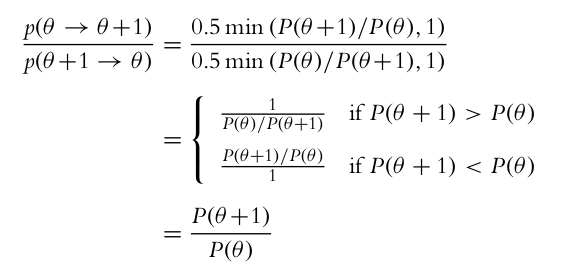
\includegraphics[scale=0.4]{pics/trans_ratio.png}
	\end{figure} 

\end{itemize}


} 
\end{frame}


\begin{frame}{Why it works}
\scriptsize{

\begin{itemize}
\item The last equation tells us that during transitions back and forth between adjacent positions, the relative probability of the transitions exactly matches the relative values of the target distribution. 
\item That might be enough to get the intuition that, in the
long run, adjacent positions will be visited proportionally to their relative values in the target distribution. 
\item If that's true for adjacent positions, then, by extrapolating from one position to the next, it must be true for the whole range of positions.

\item In more mathematical terms, this means that the transition probabilities form a Markov chain that has the target distribution as its equilibrium or stationary distribution. \cite{wiki:Markov_chain_Monte_Carlo}

\item Hence, one can obtain a sample of the desired distribution by recording states from the chain.


\end{itemize}


} 
\end{frame}


\begin{frame}{The Metropolis Algorithm more Generally}
\scriptsize{

\begin{itemize}
\item So far, we have only considered the case with a single discrete parameter $\theta$ that can only move to the left or right.

\item The general Metropolis algorithm allows working with multiple continuous parameters $\theta_1,\theta_2,\dots,\theta_n$ and more general proposal distributions.  


\item The essentials of the general method are the same as for the simple case. 

\item First, we have some target distribution $P(\theta)$ ($\theta$ can be a vector of parameters) from which we would like to generate representative sample values. 

\item We must be able to compute the value of $P(\theta)$ for any candidate value of $\theta$. 
\item The distribution, $P(\theta)$, does not have to be normalized, however. 

\item Just needs needs to be nonnegative. 


\end{itemize}


} 
\end{frame}


\begin{frame}{The Metropolis Algorithm more Generally}
\scriptsize{

\begin{itemize}

\item In our Bayesian inference application $P(\theta)$ is the unnormalized posterior distribution on  $\theta$, which is the product of the likelihood and the prior: $f(d|\theta)*f(\theta)$.

\item This is a very important property of MCMC, as it allows us to draw samples from the posterior without having to calculate the evidence $f(d)$.

\item Sample values from the target distribution are generated by taking a random walk through the parameter space.

\item Proposal distributions can take many different forms,  the goal being to use a proposal distribution
that efficiently explores the regions of the parameter space where $P(\theta)$ has most of its probability area. 

\item The generic case is using a Gaussian distribution  centered at the current position. 

\item So the proposed move will typically be near the current position, with the probability of proposing a more distant position dropping off according to the normal curve.

\item For multivariate target distributions, we can use a Multi-variate Gaussian to propose multi-dimensional points in each step. 


\end{itemize}


} 
\end{frame}


\begin{frame}{Gibbs Sampling}
\scriptsize{

\begin{itemize}

\item The Metropolis algorithm works whenever the probability of proposing a jump to B from A is equal to the probability of proposing A from B, when the proposal distribution is symmetric (such as a Gaussian distribution). 

\item There is a more general method, known as Metropolis-Hastings, that allows asymmetric proposals.

\item This would mean, that the politician's coin were biased to lead him clockwise on average.

\item Asymmetric proposal distributions allows us to explore the posterior distribution more efficiently (i.e., acquire a good image of the posterior distribution in fewer steps).

\item Gibbs sampling is a variant of the Metropolis-Hastings algorithm that uses clever proposals and is therefore more efficient.

\item The improvement arises from adaptive proposals in which the distribution of proposed parameter values adjusts itself intelligently, depending upon the parameter values at the moment.


\end{itemize}


} 
\end{frame}


\begin{frame}{Gibbs Sampling}
\scriptsize{

\begin{itemize}

\item How Gibbs sampling computes these adaptive proposals depends upon using conjugate combinations of priors and likelihoods (such as the Beta and the Binomial). 

\item As previously presented, conjugate combinations have analytical solutions for the posterior distribution of an individual parameter. 

\item And these solutions are what allow Gibbs sampling to make smart jumps around the joint posterior distribution of all parameters.

\item The algorithm works as follows:

\item At each point in the walk, the parameters are selected in an iterative cycle: $\theta_1, \theta_2, \theta_3 , \dots \theta_1, \theta_2, \theta_3, \dots.$ 

\item Suppose that parameter $\theta_i$ has been selected.

\item Gibbs sampling then chooses a new value for that parameter by generating a random value directly from
the conditional probability distribution of that parameter given all the others and $d$: 

\begin{displaymath}
f(\theta_i | \theta_1,\dots, \theta_{i-1}, \theta_{i+1}, \dots,\theta_n,d)  
\end{displaymath}





\end{itemize}


} 
\end{frame}


\begin{frame}{Gibbs Sampling}
\scriptsize{

\begin{itemize}

\item Since we are using conjugate combinations, this conditional distribution has a closed form that facilitates the sampling of random numbers from it.

\item The new value for $\theta_i$ , combined with the unchanged values of $\theta_1,\dots, \theta_{i-1}, \theta_{i+1}, \dots,\theta_n$, constitutes the new position in the random walk.

\item The process then repeats: select the next parameter $\theta_{i+1}$ and select a new value for that parameter from its conditional posterior distribution.

\item Let's illustrate this process for a two-parameter example: $\theta_1,\theta_2$.

\item In the first step, we want to select a new value for $\theta_1$ . 

\item We conditionalize on the values of all the other
parameters from the previous step in the chain. 

\item In this example, there is only one other parameter, namely $\theta_2$.


\end{itemize}


} 
\end{frame}



\begin{frame}{Gibbs Sampling}
\scriptsize{


 \begin{figure}[h!]
	\centering
	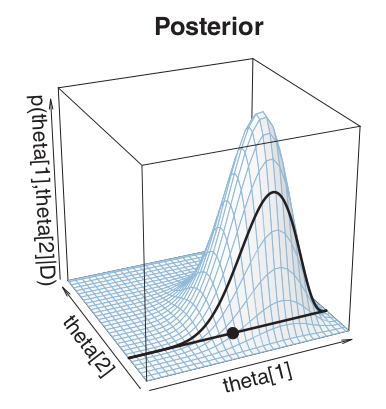
\includegraphics[scale=0.4]{pics/gibbs1.png}
	\end{figure} 

\begin{itemize}

\item The figure shows a slice through the joint distribution at the current value of $\theta_2$. 

\item The heavy curve is the posterior distribution conditional on this value of $\theta_2$, which is $f(\theta_1|\theta_2 , d)$ in this case because there is only one other parameter.

\end{itemize}


} 
\end{frame}


\begin{frame}{Gibbs Sampling}
\scriptsize{


\begin{itemize}

\item Because we are using conjugate distributions a computer can directly generate a random  value of $\theta_1$ from $f(\theta_1|\theta_2 , d)$. 

\item Having generated a new value for $\theta_1$, we then conditionalize on it and determine the conditional distribution of the next parameter, $\theta_2$ using $f(\theta_2|\theta_1 , d)$  as shown below:

 \begin{figure}[h!]
	\centering
	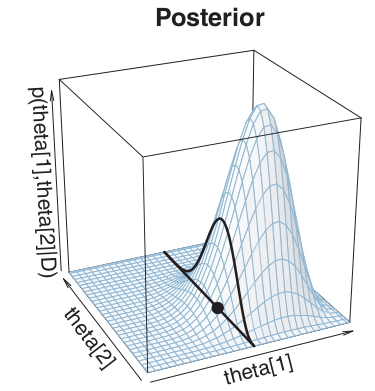
\includegraphics[scale=0.4]{pics/gibbs2.png}
	\end{figure} 

\item We generate a new value of $\theta_2$ , and the cycle repeats.



\end{itemize}


} 
\end{frame}


\begin{frame}{Gibbs Sampling}
\scriptsize{

\begin{itemize}

\item Because the proposal distribution exactly mirrors the posterior probability for that parameter, the proposed move is always accepted.

\item Hence, the algorithm is more efficient than the standard Metropolis algorithm in which proposals are rejected in many cases.

\item But there are some limitations to Gibbs sampling.

\item First, there are cases when we don't want to use conjugate priors. 

\item Second, it can become inefficient with complex models containing hundreds, thousands or tens of thousands of parameters.


\end{itemize}


} 
\end{frame}



\begin{frame}{Hamiltonian Monte Carlo}
\scriptsize{

\begin{itemize}
\item The Metropolis algorithm and Gibbs sampling are both highly random procedures.
\item They try out new parameter values and see how good they are, compared to the current values.
\item But Gibbs sampling gains efficiency by reducing this randomness and exploiting knowledge of the target distribution. 

\item Hamiltonian Monte Carlo (or Hybrid Monte Carlo, HMC) is another sampling method that is much more computationally costly than the others but its proposals are much more efficient.

\item As a result, it doesn't need as many samples to describe the posterior distribution. 
\item And as models become more complex (thousands or tens of thousands of parameters) HMC can really outshine other algorithms.

\end{itemize}


} 
\end{frame}


\begin{frame}{Hamiltonian Monte Carlo}
\scriptsize{

\begin{itemize}
\item HMC is a very complex algorithm and we won't get into the details of its inner workings

\item Let's try to understand it in a very superficial way by using again the politician's tale.

\item Suppose the politician has moved to the mainland now.

\item Now, instead of moving over a set of discrete islands, it has to move through a continuous territory stretched out along a narrow valley, running north-south.  

\item The obligations are the same: to visit his citizens in proportion to their local density.

\item And again, the politician doesn't know the population of each area in advance.

\end{itemize}


} 
\end{frame}


\begin{frame}{Hamiltonian Monte Carlo}
\scriptsize{

\begin{itemize}
\item The strategy of the politician is the following:

\item He drives his car across the narrow valley back and forth along its length.

\item In order to spend more time in densely settled areas, he slows down his  vehicle when houses grow
more dense. 
\item Likewise, he speeds up when houses grow more sparse. 
\item This strategy requires knowing how quickly population density is changing, at their current location. 

\item But it doesn't require remembering where they've been or knowing the population distribution anyplace else.

\item This story is analogous to how Hamiltonian Monte Carlo works.

\end{itemize}


} 
\end{frame}


\begin{frame}{Hamiltonian Monte Carlo}



 \begin{figure}[h!]
	\centering
	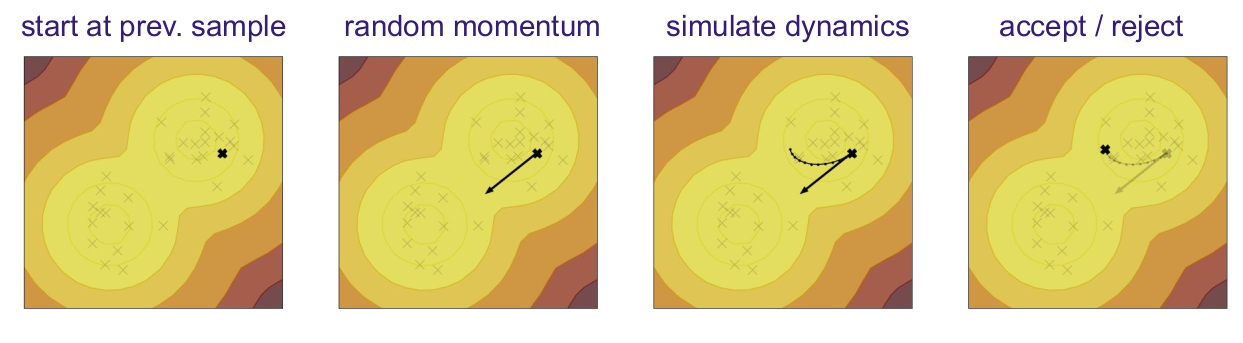
\includegraphics[scale=0.3]{pics/HMC.png}
	\end{figure} 



\end{frame}


\begin{frame}{Hamiltonian Monte Carlo}
\scriptsize{

\begin{itemize}
\item In statistical applications, the politician's vehicle is the current vector of parameter values. 


\item HMC really does run a physics simulation, pretending the vector of parameters gives the position of a little frictionless particle. 

\item The log-posterior provides a surface for this particle to glide across. 


\item Then the job is to sweep across this surface, adjusting speed in proportion to how high up we are.



\item When the log-posterior is very flat, then the particle can glide for a long time before the slope (gradient) makes it turn around.

\item When instead the log-posterior is very steep, then the particle doesn’t get far before turning around.

\end{itemize}


} 
\end{frame}


\begin{frame}{Hamiltonian Monte Carlo}
\scriptsize{

\begin{itemize}
\item A big limitation of HMC is that it needs to be tuned to a particular model and its data.


\item Stan\footnote{\url{https://mc-stan.org/}} is a very popular platform for statistical modeling and high-performance statistical computation.


\item Stan automates much of that tuning.



\item Next, we will see how to use Stan to fit a linear model with an interaction. 

\item Make sure that the \textbf{rstan} package is installed to access Stan from within R.

\end{itemize}


 \begin{figure}[h!]
	\centering
	
\includegraphics[scale=0.2]{pics/stan.png}
	\end{figure} 


} 
\end{frame}

\begin{frame}{Easy HMC: ulam}
\scriptsize{

\begin{itemize}
\item Stan provides its own language to delcare models.

\item  The rethinking package provides a convenient interface, \textbf{ulam}, to compile lists of formulas, like the lists we've been using so far to construct quap estimates, into Stan HMC
code.

\item All that ulam does is translate formulas into  Stan models, and then Stan defines
the sampler and does the hard part.

\item Stan models look very similar, but require some more explicit definitions.

\item We will show them later.

\item Before using ulam we must preprocess any variable transformations (log, exp, etc).

\item We also must construct a clean data list with only the variables we will use.



\end{itemize}




} 
\end{frame}


\begin{frame}{A model of ruggedness}
\scriptsize{

\begin{itemize}
\item We are are going to work with the \textbf{rugged} dataset from the rethinking package.
\item Each row in these data is a country, and the various columns are economic, geographic, and
historical features. 
\item The variable rugged is a Terrain Ruggedness Index that quantifies the topographic heterogeneity of a landscape. 

\item The outcome variable of our regression model will be the logarithm of real gross domestic product per capita, from the year 2000, \textbf{rgdppc\_2000}.

\item Ruggedness is usually associated with poorer countries, in most of the world.

\item Rugged terrain usually means transport is difficult, which means market access is hampered, which means reduced gross domestic product.

\item However, this associated gets inverted for African countries.


\end{itemize}




} 
\end{frame}


\begin{frame}[fragile]{A model of ruggedness}
\scriptsize{

\begin{itemize}
\item Let's load and explore the data:

\begin{verbatim}
library(rethinking)
data(rugged)
d <- rugged
d$log_gdp <- log(d$rgdppc_2000)
#remove rows with missing values
dd <- d[ complete.cases(d$rgdppc_2000) , ]
# discard columns we are not going to use
dd.trim <- dd[ , c("log_gdp","rugged","cont_africa") ]
summary(dd.trim)

> summary(dd.trim)
    log_gdp           rugged        cont_africa    
 Min.   : 6.146   Min.   :0.0030   Min.   :0.0000  
 1st Qu.: 7.539   1st Qu.:0.4422   1st Qu.:0.0000  
 Median : 8.578   Median :0.9795   Median :0.0000  
 Mean   : 8.517   Mean   :1.3332   Mean   :0.2882  
 3rd Qu.: 9.480   3rd Qu.:1.9572   3rd Qu.:1.0000  
 Max.   :10.965   Max.   :6.2020   Max.   :1.0000 
\end{verbatim}

\item Note that we do not convert cont\_africa into a factor because that produces numerical problems with the rethinking methods.

\end{itemize}




} 
\end{frame}



\begin{frame}[fragile]{A model of ruggedness}
\scriptsize{

\begin{itemize}
\item We have a dataset with countries as rows and 3 columns: 

\begin{enumerate}
\scriptsize{
 \item log\_gdp: the log GDP of the country in year 2000.
 \item rugged: the Terrain Ruggedness Index of the country
 \item cont\_africa: a binary variable (1 for African countries and 0 for non-African ones).}
\end{enumerate}


\item Let's compute the correlation between log\_gdp and rugged:

\begin{verbatim}
> cor(dd.trim$rugged,dd.trim$log_gdp)
[1] 0.002833496 
\end{verbatim}

\item It is very low. Now let's calculate them separately for African and non-African countries:

\begin{verbatim}
> dd.A<-dd.trim[dd.trim$cont_africa==1,]
> cor(dd.A$rugged,dd.A$log_gdp)
[1] 0.2607532
> 
> dd.NA<-dd.trim[dd.trim$cont_africa==0,]
> cor(dd.NA$rugged,dd.NA$log_gdp)
[1] -0.2307945 
\end{verbatim}

\item We now observe a stronger relationship between the two variables that is reversed for African and non-African countries.

\end{itemize}




} 
\end{frame}

\begin{frame}{A model of ruggedness}
\scriptsize{

\begin{itemize}
\item We will now construct a Bayesian Linear Regression between log GDP ($y$) and terrain ruggedness ($x$) capable of incorporating the different relationships for these two groups of countries encoded by the variable $A$.
\item As we learned in a previous lecture, interactions are a convenient way to include different slopes for different categories in our data.
\item Our model will be as follows:

 \vspace{0.3cm}
 \begin{table}
 \centering
 \begin{tabular}{lr}  
$y_i \sim N(\mu_i,\sigma)$ & [likelihood] \\
$\mu_i = \beta_0 + \beta_1 x_i+ \beta_2 A_i+\beta_3*x_i*A_i$ & [linear model] \\
$\beta_0 \sim N(0,100)$ & [$\beta_0$ prior] \\
$\beta_1 \sim N(0,10)$ & [$\beta_1$ prior] \\
$\beta_2 \sim N(0,10)$ & [$\beta_2$ prior] \\
$\beta_3 \sim N(0,10)$ & [$\beta_3$ prior] \\
$\sigma \sim $ Cauchy$(0,2)$ & [$\sigma$ prior] \\
\end{tabular}
\end{table}

\item We put Gaussian priors on all $\beta$ coefficients and a Cauchy prior for $\sigma$ (a t-student with 1 degree of freedom).

\item The Cauchy distribution is heavy-tailed and has proven to be a useful prior for standard deviations (especially when restrained to postive values, taking the name of half-Cauchy). 

\end{itemize}




} 
\end{frame}


\begin{frame}[fragile]{A model of ruggedness}
\scriptsize{

\begin{itemize}
\item The R code for the model would be:

\begin{verbatim}
model<-alist(
  log_gdp ~ dnorm( mu , sigma ) ,
  mu <- b0 + b1*rugged + b2*cont_africa 
  + b3*rugged*cont_africa,
  b0 ~ dnorm(0,100),
  b1 ~ dnorm(0,10),
  b2 ~ dnorm(0,10),
  b3 ~ dnorm(0,10),
  sigma ~ dcauchy(0,2)
) 
\end{verbatim}

\item Let's try to fit this model using Laplace Approximation:

\begin{verbatim}
> b.reg3<-quap(model,data=dd.trim)
Error in quap(model, data = dd.trim) : 
  initial value in 'vmmin' is not finite
The start values for the parameters were invalid. 
\end{verbatim}

\item The optimizer is having a hard time finding the MAP estimates for this model!

\item This can sometimes be corrected by using start values (declared with the \textbf{start} parameter), but in many models even this does not help.

\end{itemize}


} 
\end{frame}

\begin{frame}[fragile]{A model of ruggedness}
\scriptsize{

\begin{itemize}
\item After trying to fit b.reg3 with quap many times, it worked!

\begin{verbatim}
> precis(b.reg3)
       mean   sd  2.5% 97.5%
b0     9.22 0.14  8.95  9.49
b1    -0.20 0.08 -0.35 -0.05
b2    -1.95 0.22 -2.39 -1.51
b3     0.39 0.13  0.14  0.65
sigma  0.93 0.05  0.83  1.03
\end{verbatim}

\item Let's interpret the mean values for the posterior marginals of each $\beta$ coefficient:

\begin{itemize}\scriptsize{
 \item mean(b0) = 9.22: this is the intercept for non-African countries.
 \item mean(b1)=-0.20: this is the slope for non-African countries, which is clearly negative.
 \item mean(b2)=-1.95: this is the difference between the intercept for African and non-African countries, which indicates that African countries have a lower GDP than non-African countries when rugedness is zero.
\item mean(b3)=0.39: this is the difference between the slopes for African and non-African countries, which indicates that the slope for non-African countries is positive (0.39-0.2).
}
 \end{itemize}


\end{itemize}


} 
\end{frame}

\begin{frame}[fragile]{Ulam}
\scriptsize{

\begin{itemize}
\item Now, let's fit the same model using Stan HMC with \textbf{ulam}:

\begin{verbatim}
m.reg1 <- ulam(model ,data=dd.trim) 
\end{verbatim}



\item After messages about compiling, and sampling, ulam returns an object that contains a
bunch of summary information, as well as samples from the posterior distribution.

\item This process takes much longer than our previous quap estimates.

\item We can summarize just like with quap:

\begin{verbatim}
> precis(m.reg1, prob=0.95 )
       mean   sd  2.5% 97.5% n_eff Rhat4
b0     9.21 0.15  8.89  9.51   169  1.03
b1    -0.20 0.09 -0.37 -0.01   163  1.04
b2    -1.95 0.23 -2.37 -1.48   241  1.01
b3     0.39 0.13  0.10  0.66   243  1.03
sigma  0.95 0.05  0.85  1.06   348  1.00
\end{verbatim}

\item These estimates are very similar to the Laplace approximation.


\end{itemize}




} 
\end{frame}


\begin{frame}[fragile]{Ulam}
\scriptsize{

\begin{itemize}

\item There are two new columns, n\_eff and Rhat, which provide MCMC diagnostic criteria, to help us tell how well estimation worked. 

\item The column n\_eff is a crude estimate of the number of independent samples we managed to get.

\item Rhat  is the Gelman Rubin convergence diagnostic, which estimates  the convergence of the Markov chains to the target distribution.

\item It should approach 1.00 from above, when all is well.


 \end{itemize}







} 
\end{frame}


\begin{frame}[fragile]{Ulam}
\scriptsize{

\begin{itemize}

\item A report of the chain can be obtained with command \textbf{show}:
\begin{verbatim}
> show(m.reg1)
Hamiltonian Monte Carlo approximation
500 samples from 1 chain

Sampling durations (seconds):
        warmup sample total
chain:1    0.2   0.17  0.37

Formula:
log_gdp ~ dnorm(mu, sigma)
mu <- b0 + b1 * rugged + b2 * cont_africa +
b3 * rugged * cont_africa
b0 ~ dnorm(0, 100)
b1 ~ dnorm(0, 10)
b2 ~ dnorm(0, 10)
b3 ~ dnorm(0, 10)
sigma ~ dcauchy(0, 2) 
\end{verbatim}



 \end{itemize}







} 
\end{frame}

\begin{frame}[fragile]{Stan Code}
\scriptsize{

 We can also get the Stan code with: \verb+stancode(m.reg1)+:  
\begin{verbatim}
data{
    vector[170] log_gdp;
    int cont_africa[170];
    vector[170] rugged;
}
parameters{
    real b0;
    real b1;
    real b2;
    real b3;
    real sigma;
}

\end{verbatim}


} 
\end{frame}


\begin{frame}[fragile]{Ulam}
\scriptsize{

 
\begin{verbatim}

model{
    vector[170] mu;
    sigma ~ cauchy( 0 , 2 );
    b3 ~ normal( 0 , 10 );
    b2 ~ normal( 0 , 10 );
    b1 ~ normal( 0 , 10 );
    b0 ~ normal( 0 , 100 );
    for ( i in 1:170 ) {
        mu[i] = b0 + b1 * rugged[i] + b2 * cont_africa[i] 
        + b3 * rugged[i] * cont_africa[i];
    }
    log_gdp ~ normal( mu , sigma );
}

\end{verbatim}

This is Stan code, not R code. It is essentially the formula list we provided to ulam , but in reverse order.

} 
\end{frame}


\begin{frame}[fragile]{Ulam}
\scriptsize{


\begin{block}{Additional Ulam Parameters}
\begin{itemize}


\item \textbf{iter}: the number of samples from the chain. The default is 1000.
\item \textbf{warmup}: the number of tuning samples. These samples are used to adapt sampling, and so are not actually part of the target posterior distribution. The default value is iter/2 , which gives us 500 warmup samples and 500 real samples to use for inference.

\item \textbf{chains}: the number of independent Markov chains to sample from. All of the non-warmup samples from each chain will be automatically combined in the resulting inferences.

\item \textbf{cores}: the number of procesors over which the chains will be distributed.



 \end{itemize}

 \end{block}

\begin{itemize}


\item Let's fit the same model sampling 4 different chains distributed over 4 CPU cores with 3000 iterarions and 1000  warmups.

\begin{verbatim}
m.reg2 <- ulam(model ,data=dd.trim, iter=3000, 
               warmup =1000, chains=4, cores=4) 

show(m.reg2) 
\end{verbatim}


 \end{itemize}




} 
\end{frame}


\begin{frame}[fragile]{Ulam}
\scriptsize{


\begin{itemize}


\item Let's fit the same model sampling 4 different chains distributed over 4 CPU cores with 3000 iterarions and 1000  warmups.

\begin{verbatim}
> m.reg2 <- ulam(model ,data=dd.trim, iter=3000, 
               warmup =1000, chains=4, cores=4) 
> show(m.reg2)
Hamiltonian Monte Carlo approximation
8000 samples from 4 chains

Sampling durations (seconds):
        warmup sample total
chain:1   0.62   1.08  1.70
chain:2   0.54   1.06  1.60
chain:3   0.60   0.89  1.49
chain:4   0.37   0.82  1.19

\end{verbatim}


 \end{itemize}




} 
\end{frame}


\begin{frame}[fragile]{Ulam}
\scriptsize{


\begin{itemize}


\item We can extract samples from the posterior in the usual way:

\begin{verbatim}
post <- extract.samples( m.reg1 )
\end{verbatim}

\item We also use \textbf{link} and \textbf{sim} functions to get posterior predictions.

\item  We can plot the correlations between samples using the function \textbf{pairs}:

\begin{verbatim}
pairs( m.reg1)
\end{verbatim}

\item This will show a pairs plot: a matrix of bivariate scatter plots. \item Along the diagonal the smoothed histogram of each parameter is shown, along with its name.
\item In in the lower triangle of the matrix, below the diagonal, the correlation between each pair of parameters is shown, with stronger correlations indicated by relative size.

 \end{itemize}




} 
\end{frame}


\begin{frame}{Ulam Pairs}



 \begin{figure}[h!]
	\centering
	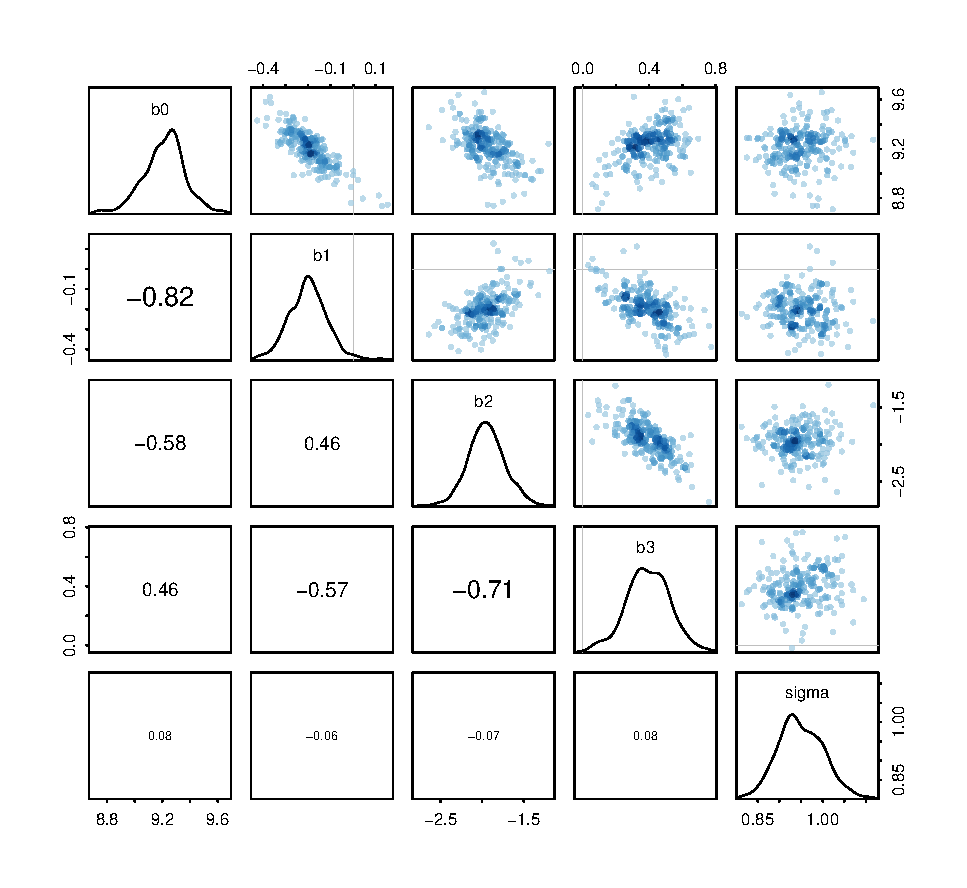
\includegraphics[scale=0.55]{pics/MCMC_pairs.pdf}
	\end{figure} 



\end{frame}


\begin{frame}[fragile]{Ulam Pairs}
\scriptsize{


\begin{itemize}


\item For this model and these data, the resulting posterior distribution is quite nearly multivariate Gaussian.
\item The density for sigma is certainly skewed in the expected direction. \item But otherwise the Lapalce approximation does almost as well as Hamiltonian Monte Carlo.
\item This is a very simple kind of model structure of course, with Gaussian priors, so an approximately Gaussian posterior should be no surprise. 
\item For more complex models, posterior distributions take more exotic shapes.

 \end{itemize}




} 
\end{frame}


\begin{frame}[fragile]{Checking the Chain }
\scriptsize{


\begin{itemize}


\item Provided the Markov chain is defined correctly then it is guaranteed to converge in the long run to the answer we want, the posterior distri-
bution. 
\item But the machine does sometimes malfunction.

\item We won't study these cases in detail.

\item A trace plot is a very useful tool for diagnosing malfunction.

\item It basically plots the samples in sequential order, joined by a line.

\item In the terrain ruggedness example, the trace plot shows a very healthy chain.

\item We can obtain it with the following command:

\begin{verbatim}
traceplot( m.reg1 ) 
\end{verbatim}


 \end{itemize}




} 
\end{frame}


\begin{frame}{Trace Plot}



 \begin{figure}[h!]
	\centering
	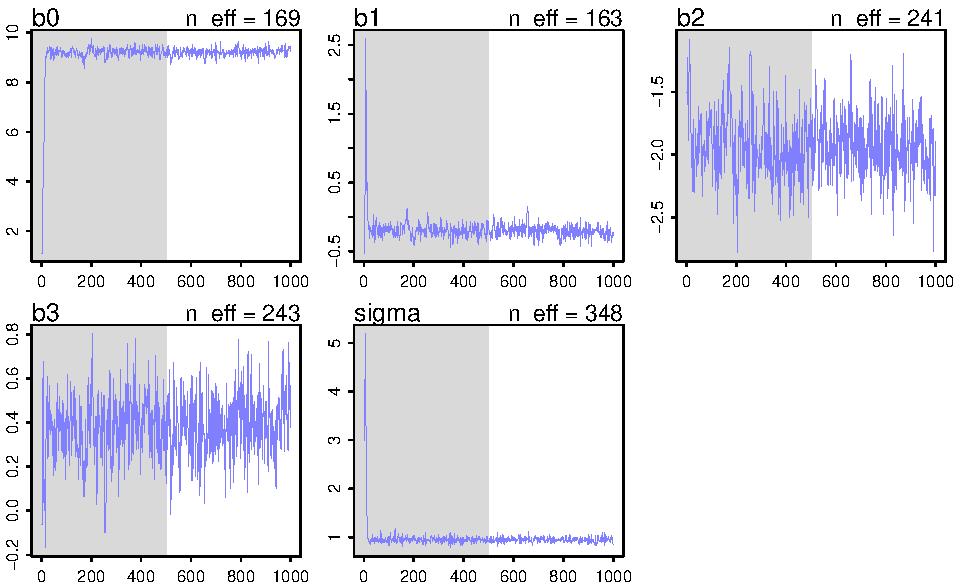
\includegraphics[scale=0.7]{pics/traceplot.pdf}
	\end{figure} 



\end{frame}


\begin{frame}[fragile]{Checking the Chain }
\scriptsize{


\begin{itemize}


\item The plot shows the zig-zagging trace of each parameter as the path the chain took through each dimension of parameter space.

\item The gray region in each plot, the first 500 samples, marks the warmups samples.

\item During adaptation, the Markov chain is learning to more efficiently sample from the posterior distribution.

\item So these samples are not necessarily reliable to use for inference. 
\item They are automatically discarded by \textbf{extract.samples} , which returns only the samples shown in the white regions.


\item Typically we look for two things in these trace plots: stationarity and good mixing. 

 \end{itemize}




} 
\end{frame}


\begin{frame}[fragile]{Checking the Chain }
\scriptsize{


\begin{itemize}


\item Stationarity refers to the path staying within the poste-
rior distribution. 

\item Notice that these traces, for example, all stick around a very stable central tendency, the center of gravity of each dimension of the posterior.

\item Another way to think of this is that the mean value of the chain is quite stable from beginning to end.

\item A well-mixing chain means that each successive sample within each parameter is not highly correlated with the sample before it.

\item Visually, you can see this by the rapid zig-zag motion of each path, as the trace traverses the posterior distribution without getting mired
anyplace.

 \end{itemize}




} 
\end{frame}

\begin{frame}{Conclusions}
\scriptsize{

\begin{itemize}
\item This class has been an  introduction to Markov chain Monte Carlo (MCMC) estimation. 

\item The goal has been to introduce the purpose and approach MCMC algorithms.
\item The major algorithms introduced were the Metropolis, Gibbs sampling, and Hamiltonian
Monte Carlo algorithms.
\item Each has its advantages and disadvantages. 
\item A function in the rethinking package, ulam , was introduced that uses the Stan Hamiltonian Monte Carlo engine to a linear model with an interaction.
\end{itemize}


} 
\end{frame}


%%%%%%%%%%%%%%%%%%%%%%%%%%%
\begin{frame}[allowframebreaks]\scriptsize
\frametitle{References}
\bibliography{bio}
\bibliographystyle{apalike}
%\bibliographystyle{flexbib}
\end{frame}  









%%%%%%%%%%%%%%%%%%%%%%%%%%%

\end{document}
